\section{Volta 架构白皮书阅读}

前几章中，我们已详细探讨了英伟达白皮书中常见的关键参数。在深入探讨 Volta 架构之前，回顾前几章的内容非常重要——它们
奠定了理解本章主题所必需的基础知识。熟悉这些参数至关重要，因为我们将在本章中引用并验证它们。

现在就来看看 Volta 架构的规格。打开 Volta 白皮书（即 V100 白皮书），你可以在开头看到目录。在目录的第二页，你会找到一
个名为"关键特性"的部分。这不仅仅是一系列改进的列表，更是 V100 相比前代架构重大增强的全面概述。

点击"关键特性"标题后，我们将看到定义 V100 GPU 即 Volta 架构的核心特性，从新的 SM 设计到第二代 NVLink 技术等。
本章将逐一讨论所有这些增强功能。回到目录，这份白皮书的一个突出方面是专门聚焦于人工智能和深度学习。考虑到 Volta 架构首
次引入了张量核心（Tensor Core），这种对 AI 和深度学习的聚焦是十分自然的。

\begin{figure}
    \centering
    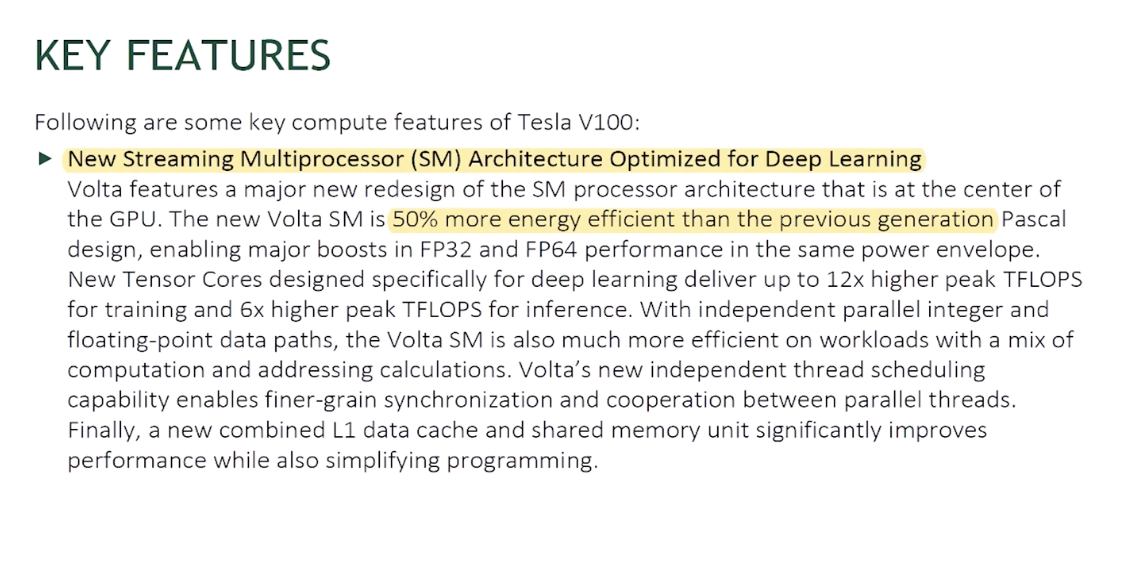
\includegraphics[width=0.75\linewidth]{resources/cuda-049.png}
    \caption{Volta 架构关键特性}
    \label{fig:placeholder}
\end{figure}

\begin{figure}
    \centering
    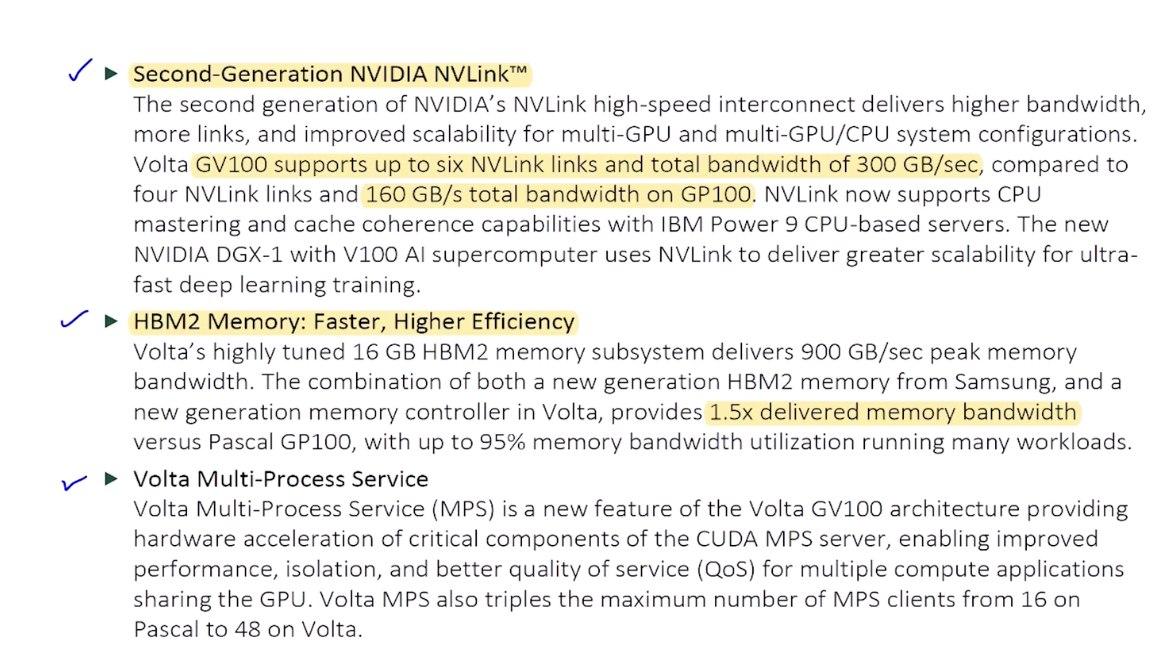
\includegraphics[width=0.75\linewidth]{resources/cuda-050.png}
    \caption{Volta 架构关键特性}
    \label{fig:placeholder}
\end{figure}


\subsection{Volta关键特性}

张量核心是专门设计用来执行矩阵运算的计算单元，这对神经网络的训练和推理阶段至关重要，也是 Volta 架构的重大突破。请注
意目录中“深入硬件架构”这个关键标题。这一标题并非 Volta白皮书独有，它在英伟达各款白皮书中反复出现。例如，Pascal 白皮书和最近的 Hopper (H100)白皮书目录中都有相同的术语。
这提醒了我们之前讨论过的重要一点：尽管每份白皮书详述不同的架构，但英伟达白皮书采用了相似的结构方法。此外，Volta白皮书还包含软件增强部分以及提供其他设备详细信息的附录。

现在，让我们深入浏览白皮书。文中提到 V100 GPU 拥有约 210 亿个晶体管。作为对比，H100 包含 800亿个
晶体管。这意味着从 Volta 到 Hopper，晶体管数量增加了近 4 倍。晶体管数量是可用的计算资源指标，更多的晶体管
通常对应硬件单元数量的增加。

\subsection{SM增强}

接下来讨论 Volta 架构的关键特性和增强。首先是 \textbf{SM 增强}：


\begin{figure}
    \centering
    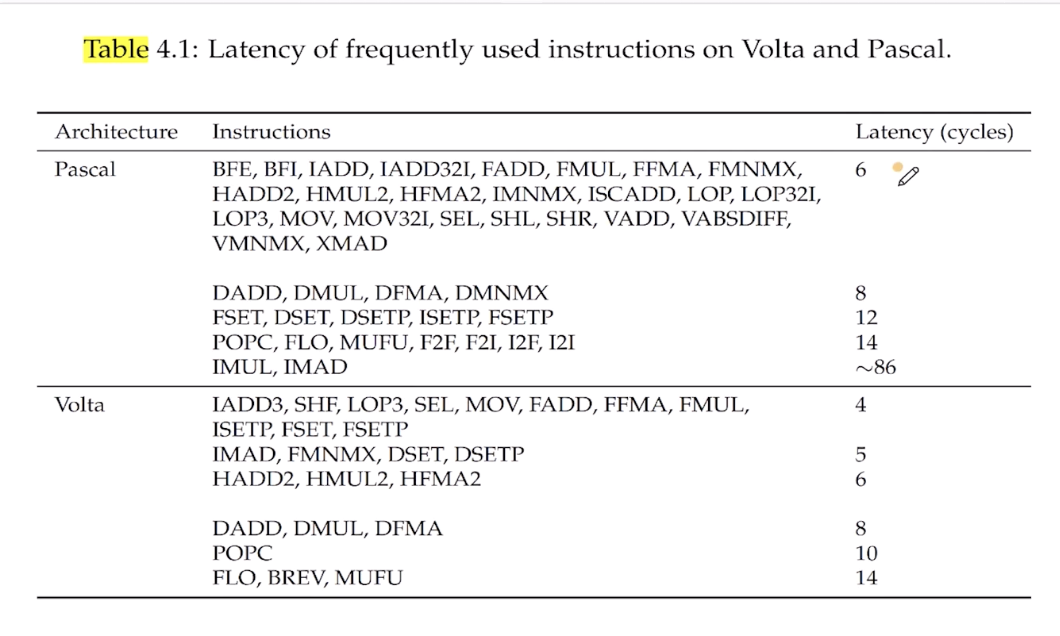
\includegraphics[width=0.75\linewidth]{resources/cuda-051.png}
    \caption{Volta 单精度和双精度核心改进}
    \label{fig:placeholder}
\end{figure}


\begin{enumerate}
    \item \textbf{能效提升}：Volta 的新 SM 设计比前代 Pascal 架构能效高出 50\%。对于管理大规模计算系统的企业来说，这意味着 V100 有可能将能源成本减半，且不牺牲计算能力。

    \item \textbf{单精度和双精度核心改进}：在功耗不变的情况下，新 SM 为 FP32（单精度）和 FP64（双精度）性能提供了重大改进。研究论文中的指令延迟对比表显示，Pascal 中加法/减法指令需要 6 个周期，而 Volta 仅需 4 个周期。后续的 Ampere 架构进一步降至 2 个周期。这说明英伟达不仅增加了核心数量，也在不断提升现有单元的执行速度。

    \item \textbf{用于 AI 计算的张量核心}：这是新 SM 中的全新单元，能为神经网络训练带来高达 12 倍的吞吐量提升（TFLOPS），推理方面提升 6 倍。虽然张量核心的单条指令延迟在 4-8 个周期之间（取决于矩阵形状和数据类型），但它们是在矩阵级别而非单个元素上执行操作，从而实现了巨大的性能飞跃。

    \item \textbf{增强的整数和浮点数并行性}：在 Pascal 及更早架构中，整数和浮点运算无法同时执行。但在 Volta 的新 SM 中，每种运算都有独立路径，允许整数和浮点运算并行运行。这对于混合数据类型的现代工作负载至关重要。

    \item \textbf{高级线程调度与内存合并}：除了提升访问速度外，还将 L1 高速缓存和共享内存合并到了一个物理单元中。
\end{enumerate}

第二个架构级增强是\textbf{第二代 NVLink 技术}（稍后详述）。

第三个特性是\textbf{全局内存增强}。Volta 的内存带宽达到 900\,GB/s，而 Pascal 约为700 \,GB/s。相比之下，Ampere 架构达到了约1500\,GB/s。更高的内存带宽意味着更快的数据访问和更高的数
据处理效率。

\begin{figure}
    \centering
    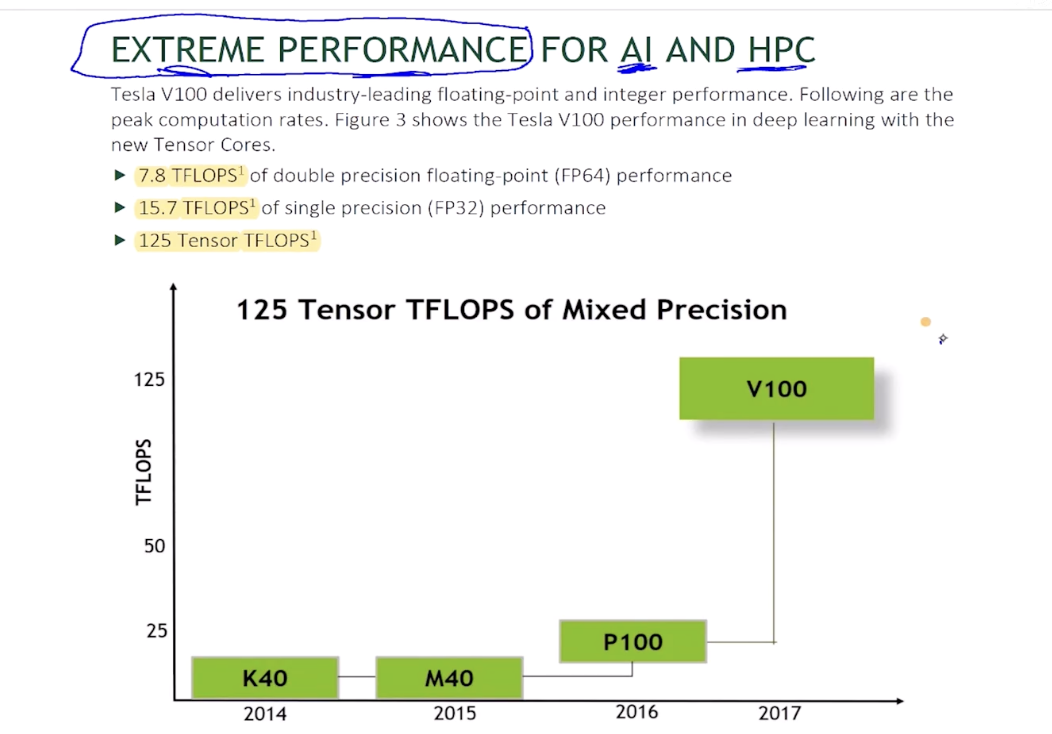
\includegraphics[width=0.75\linewidth]{resources/cuda-052.png}
    \caption{Volta 性能提升}
    \label{fig:placeholder}
\end{figure}


此外，还有\textbf{多进程服务（MPS）}，旨在优化单个 GPU上同时执行的多个应用程序的性能；以
及\textbf{统一内存}增强，将 GPU 和 CPU内存合并为单一虚拟地址空间。最后，常用的 GPU 加速计算库也进
行了更新，以有效利用这些新硬件单元。

白皮书强调了针对 AI 和高性能计算的“极致性能”。引入张量核心后，V100 实现了 125\,TFLOPS的吞吐量，相
比 Pascal 的约 21\,TFLOPS 是显著提升。

\subsection{深入硬件架构}

接下来进入最重要的部分：\textbf{深入探讨 GV100 GPU 硬件架构}。每个 GPU 包含多个 SM，每个SM
包含 L1/共享内存及各类计算单元。在 Volta 中，每个 SM 配备 64 个单精度核心、64个整数核心、32 个双
精度核心和 8 个张量核心。整个 GPU 拥有 84 个 SM，总计约有 2 万个计算单元。GPU内部还包括 6\,MB
的二级高速缓存（L2 Cache），通过内存控制器连接所有 SM，底部则是用于互联的NVLink 单元。

深入单个 SM，它由\textbf{四个分区}组成。这种分区策略允许将不同的软件块分配到不同分区并发执行，最大化资源利用
率。每个分区包含：

\begin{figure}
    \centering
    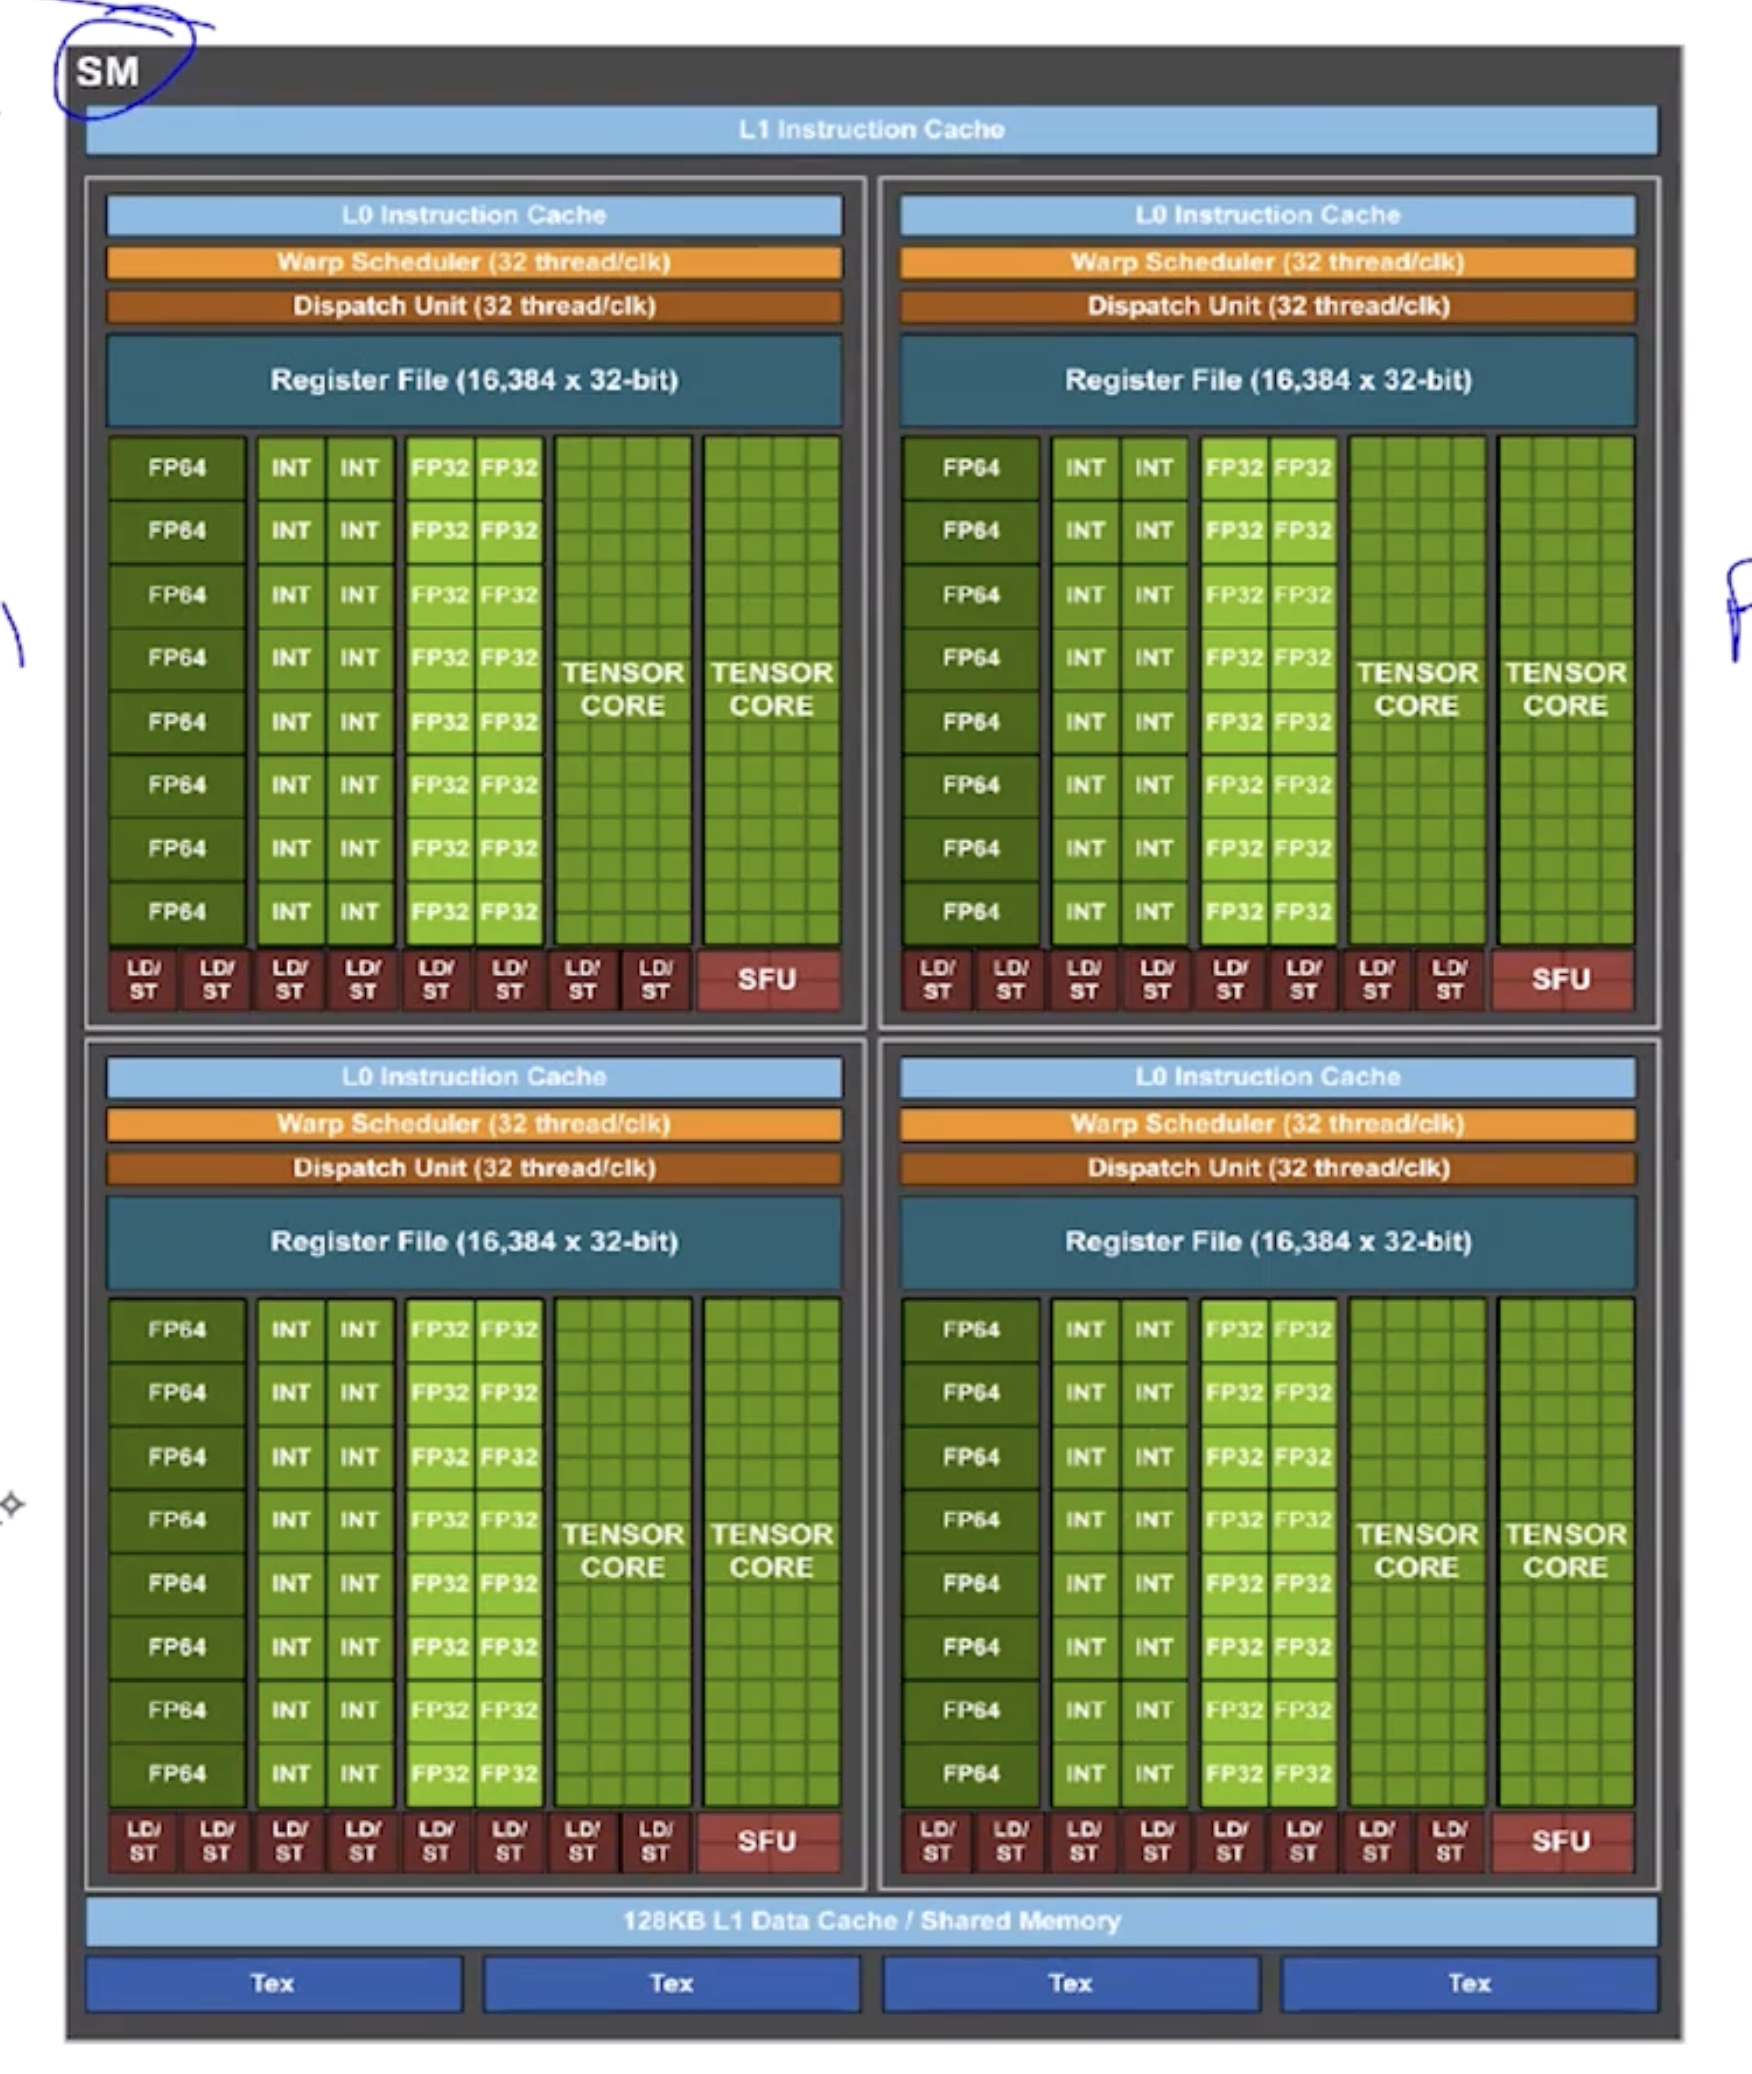
\includegraphics[width=0.75\linewidth]{resources/cuda-053.png}
    \caption{SM 内部架构}
    \label{fig:placeholder}
\end{figure}


\begin{itemize}
    \item \textbf{L0 指令高速缓存}：存储待执行指令。
    \item \textbf{Warp 调度器}：负责管理线程束（Warp，即 32 个线程为一组）。采用 SIMT（单指令多线程）模式，即一个 Warp 内的 32 个线程在不同核心上并行执行相同指令。
    \item \textbf{分发器（Dispatch Unit）}：与调度器协同，将指令分发到执行单元。
    \item \textbf{寄存器文件}：保存临时数据。
    \item \textbf{执行单元}：包括单精度/整数核心、张量核心及特殊功能单元（SFU）。
\end{itemize}

四个分区共享同一个 L1 高速缓存、共享内存和纹理内存。

\subsection{架构对比与NVLink}

让我们参考 A100 白皮书中的对比表来比较 Ampere、Volta 和 Pascal 架构：

\begin{figure}
    \centering
    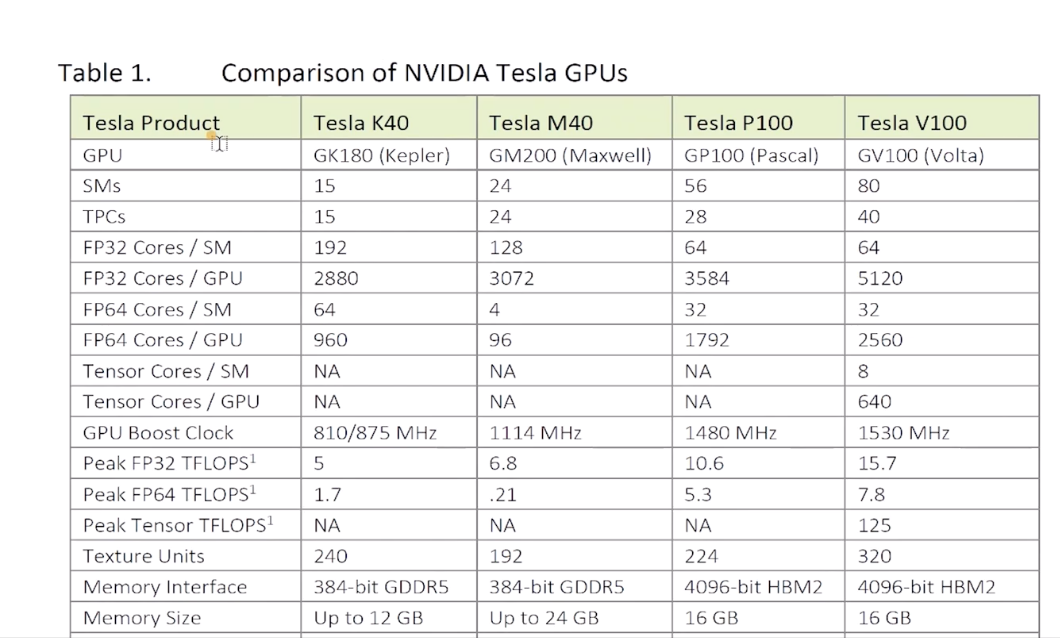
\includegraphics[width=0.75\linewidth]{resources/cuda-054.png}
    \caption{架构对比}
    \label{fig:placeholder}
\end{figure}


\begin{itemize}
    \item \textbf{SM 数量}：Pascal (56) $\rightarrow$ Volta (80) $\rightarrow$ Ampere (108)。
    \item \textbf{单精度核心}：Pascal ($\sim$3500) $\rightarrow$ Volta ($\sim$5000) $\rightarrow$ Ampere ($\sim$7000)。
    \item \textbf{整数核心}：Pascal 无独立整数核心（与浮点共用）；Volta ($\sim$5000)；Ampere ($\sim$7000)。
    \item \textbf{张量核心}：Pascal 无；Volta (640)；Ampere (432)。注意：虽然 Ampere 张量核心数量少于 Volta，但其单核能力和效率大幅提升，整体吞吐量反而是 Volta 的两倍以上。评估性能不能只看核心数量，还要看核心能力。
    \item \textbf{FP16 吞吐量（带 FP32 累加）}：Ampere 远超 Volta。这里涉及“使用单精度累加的半精度计算”概念，即输入为 FP16，但输出/累加使用 FP32 以保证精度。
    \item \textbf{常规单精度吞吐量}：Pascal (21\,TFLOPS) $\rightarrow$ Volta (31\,TFLOPS) $\rightarrow$ Ampere (78\,TFLOPS)。
    \item \textbf{显存位宽}：Volta ($\sim$4096-bit) vs Ampere ($>$5120-bit)。
    \item \textbf{显存容量}：Volta (16/32\,GB) vs Ampere (40\,GB)。
    \item \textbf{内存带宽}：Pascal ($\sim$700\,GB/s) $\rightarrow$ Volta (900\,GB/s) $\rightarrow$ Ampere (1500\,GB/s)。带宽受显存大小、速度和位宽共同影响。
    \item \textbf{L2 缓存}：Volta (6\,MB) $\rightarrow$ Ampere (40\,MB)，增长超 7 倍。
    \item \textbf{晶体管数}：Volta (210 亿) $\rightarrow$ Ampere (540 亿)。工艺从 Volta 的 12\,nm 演进到 Ampere 的 7\,nm。
\end{itemize}

\begin{figure}
    \centering
    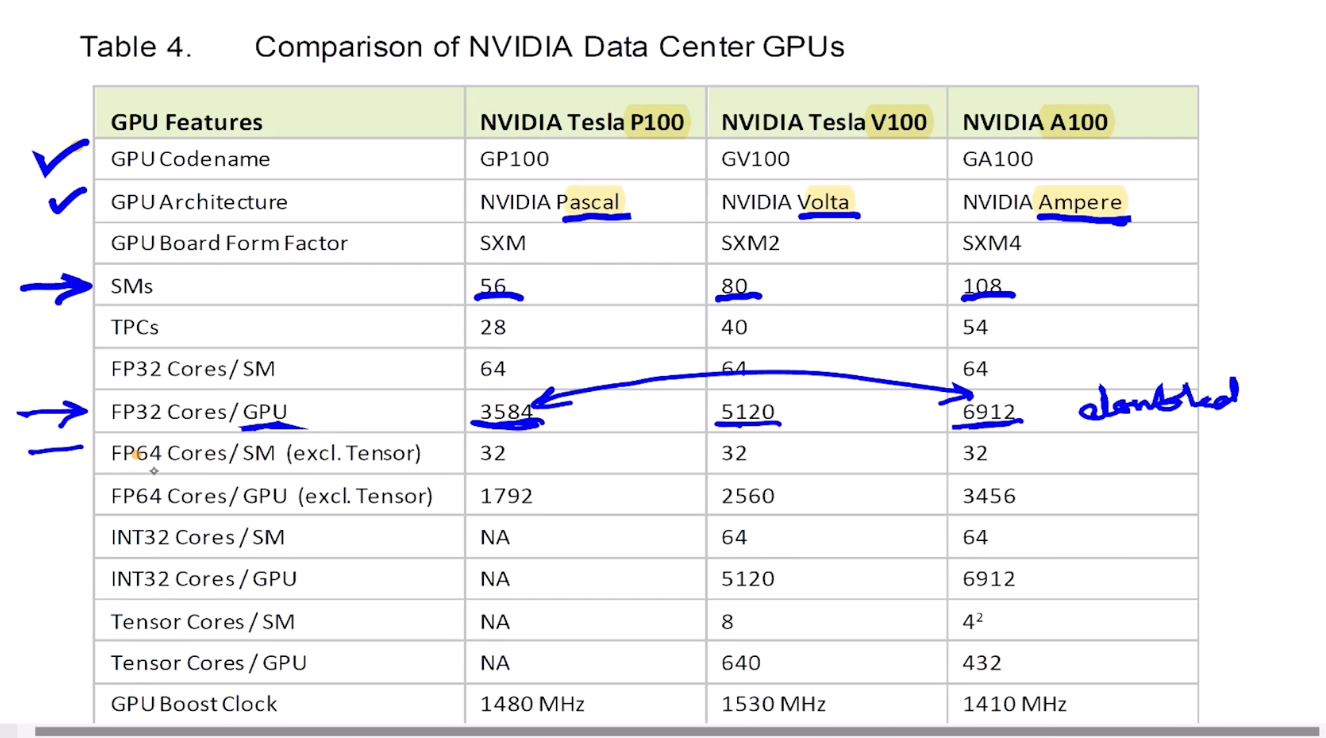
\includegraphics[width=0.75\linewidth]{resources/cuda-055.png}
    \caption{架构对比}
    \label{fig:placeholder}
\end{figure}


编写 CUDA 程序时，还需参考"CUDA 计算能力"表，了解最大线程数、最大块数等硬件限制。如果应用规模超出限制，需将其拆
分为多个核函数（kernel）执行。

\begin{figure}
    \centering
    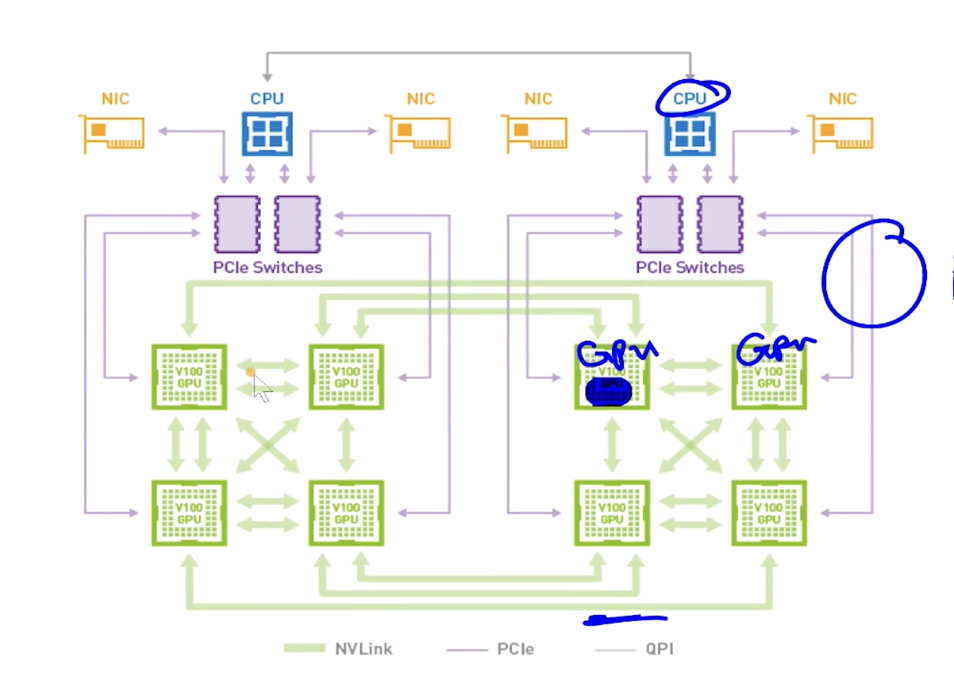
\includegraphics[width=0.75\linewidth]{resources/cuda-056.png}
    \caption{NVLink}
    \label{fig:placeholder}
\end{figure}


关于 \textbf{NVLink}：这是一种高速互联技术。第二代 NVLink 相比 Pascal的第一代有两大改进：
一是链路数量增加（GPU 间从 1 条增至 2 条以上）；二是链路速度提升。这使得 GPU间通信带宽从 Pascal 的 160\,GB/s 提升
至 Volta 的 300\,GB/s。NVLink 是 DGX服务器的标准特性。例如 DGX Station（4 块 V100）和 DGX-1（8 块 V100）。
对比 DGX-1的 Pascal 和 Volta 版本，虽然整机功耗同为 3200\,W，但 Volta版本凭借张量核心在同等能耗下提供了数倍于 Pascal 的计算性能
（能效比提升）。

本章涵盖了 Volta 架构的重点，并对比了 Pascal 和 Ampere。建议读者继续阅读白皮书剩余部分。
